\documentclass[12pt]{report}
\usepackage{graphicx}
\usepackage{pstricks}
\usepackage{pst-node}
\usepackage{pst-text}
\usepackage{etex}
\usepackage{caption}
\usepackage{pst-rel-points}
\usepackage{listings}
\usepackage[english]{babel}
\usepackage{flexiprogram}

\AtBeginDocument{\renewcommand{\bibname}{References}}

\lstset {language=C++}
  \begin{document}

\begin{titlepage}
\thispagestyle{empty}
\vspace*{0.7cm}
{\centering    
\large
{\Large\bf Bidirectional context sensitive analysis framework in PRISM}\\
\vspace{1cm}
\bf{\textit{(M. Tech Project Stage-II Report)}}\\ 
\vspace{0.75cm}
\it{Submitted in partial fulfillment of the requirements}\\
\vspace{0.5cm}
\it{of the degree of}\\
\vspace{0.5cm}
\bf{Master of Technology}\\
\vspace{0.1cm}
%\vspace{1cm}
\it
by \\
\vspace{.5cm}
\rm
{\large \bf {Vinit Deodhar}}\\
{\large \bf {(123050035)}}

\vspace{0.75cm}

{\it{under the guidance of}} \\
\vspace{.5cm}

\hspace{.05cm} {\large \bf {Prof. Uday Khedker}}\\
\vspace {0.75cm}
%\vspace {0.5cm}
%\begin{figure}[h]
%\hspace{.05cm}
%{\centering{\includegraphics[height=3.5cm,width=4.5cm]{iitb_logo.png}}\par}
%\end{figure}
\vspace{0.4cm}
Department of Computer Science and Engineering \\
Indian Institute of Technology, Bombay\\
{\centering
\hspace{5.7cm}May 2014}
}
\pagebreak
\end{titlepage}


\begin{abstract}
PRISM is an analyzer generator developed by TRDDC. Currently PRISM does not perform context sensitive interprocedural data flow analysis. Context sensitive interprocedural data flow analysis aims to improve precision of data flow analysis by incorporating effect of function calls on caller and calling context on the callee. With the long term goal of improving PRISM, this project takes two steps. Firstly we present implementation of context sensitive interprocedural data flow analysis in PRISM framework using value contexts. Secondly we aim to imrpove the specification mechanism in PRISM and studied specfication of lattices as a part of analyzer generator specifications.

\end{abstract}

\newpage
\chapter*{Acknowledgements}

I would like to take this opportunity to express gratitude to Prof Uday Khedker for his constant motivation and support. The project was supervised by TATA Research Development and Design Center (TRDDC). I am greatful to Ravindra Naik, Shrawan kumar, and Bharti C from TRDDC for their suggestions and support. Also I would like to thank my colleagues at the GCC Resource center (GRC) at IIT Bombay. Many of the ideas presented in this work are the result of our discussions.

\newpage
\tableofcontents 
\psset{unit=1mm}
\newpage
\chapter{Introduction}

Data flow analysis \cite{dfa} is a technique for gathering information about the possible set of values of some property calculated at various points in a computer program. A static data flow analysis is data flow analysis performed without executing the program. An interprocedural data flow analysis is data flow analysis across procedure boundaries. Interprocedural analysis considers only interprocedurally valid paths in the program. Due to presence of large number of contexts, many analyzers give up context sensitivity for sake of scalability and efficiency. We have implemented an interprocedural analysis framework by implementing context sensitive analysis using value contexts.

PRISM is a program analyzer generator developed by Tata Research Development and Design Center (TRDDC). Current version of PRISM does not perform context sensitive interprocedural analysis. This report presents our findings in implementation context sensitive interprocedural data flow analysis framework in PRISM analyzer generator. This report also identifies some limitations with the current version of PRISM and reviews some methods to overcome these limitations.



\section{Improving PRISM analyzer generator : Long term goals}

In this section we give an overview of the long term goals about extending PRISM analyzer generator. Following are the parameters on the lines of which we look forward to improve PRISM analyzer generator in the long run. 

\begin{enumerate}
\item Precision of data flow information : One of the goal is to implement a flow sensitive context sensitive data flow analysis. Currently PRISM uses a summary based approach for solving problems. This leds to inclusion of spurious values. This can be observed from the example program in figure \ref{fig:prog2} The summary based approach which is used in PRISM will analyze the program by solving the functions in a fixed order, eg first f and then g. While solving f, parameters passed to call to function g are marked live. Thus at the IN of function call in main the summary based approach gives \{p,q,r\} as set of live variables. It can be observed that r is never used, hence it is spuriously marked live. Interprocedural analysis will not include such variables in the data flow information and will give more precise information.

\item Usefulness of data flow information :  Only useful data flow information must be propagated. Useful information is a subset of valid data flow information. This can be done by allowing analysis to be performed in a liveness based way where only information corresponding to live variables is retained. eg : Liveness based analysis propagates information of live variables only, since it is the only useful information. The difference between precise and useful information is shown in figure \ref{fig:prog2}. Here at the IN of function call in main, the precise information is \{p,q\} since both p,q can be used after the program point. But useful information is only \{q\} because it is the only variable which will affect the behaviour of the program. variable p is used is assigned but its value does not affect the behaviour of program. Such useful live variables are called strong live variables.
\item Scalability of datflow analysis : Many analyzers compromise on flow or context sensitivity to support scalability. This is because number of contexts grow rapidly as the size of program grows. We aim to implement a scalable framework which is both context sensitive and flow sensitive.


\item Support to solve wider class of data flow analysis : Many analyzer generators in practice including PRISM solve only unidirectional data flow problems. We plan to add support for solving bidirectional data flow analysis problems.
\item Concise and easy to learn specifications : Learning current kulang specifications used in PRISM is a steep learning curve. Moreover meet functions need to be user defined which increases the complexity as well as chance of an error. 
\item Ease of debugging and testing : An error in kulang specifications gets propagated into generated code and is not easy to debug. We aim to create a system where any errors in kulang specifications are easy to track and debug.
\end{enumerate}

\begin{figure}[!ht]
\begin{pspicture}(0,0)(150,150)

\begin{psframe}(0,0)(145,150)
\putnode{n1}{origin}{30}{75}{\psframebox[linestyle=none]{\begin{tabular}{@{}l@{}}
$void~f(int~m,int~n,int~o)$\\
$\{$\\
$~$\\
$~~int~a;$\\
$~~if(a)$\\
$~~~~~g(m,n);$\\
$~~print~n$\\
$~~a=m$\\
$\}$\\
$~$\\
$void~g(int~x,int~y,int~z)$\\
$\{$\\
$~$\\
$~~int~b;$\\
$~~if(b)$\\
$~~~~f(x,y,z);$\\
$~~print~y$\\
$~~b=x$\\
$\}$\\
$~$\\
$int~main()$\\
$\{$\\
$~$\\
$~~int~p,q,r;$\\
$~~f(p,q,r);$\\
$~~return~0;$\\
$\}$\\
$~$\\
\end{tabular}}}

\end{psframe}

\end{pspicture}
\caption{Precise and useful liveness information}
\label{fig:prog2}
\end{figure}


\section{Value addition done by this project}

In the direction of the long term goals, the value addition done by this project is implementation of a interprocedural unidirectional data flow analysis framework in PRISM using value contexts. This will help in improving the precision of data flow values. An analysis for liveness and strong liveness was implemented and performance measurements were taken to measure various parameters of PRISM analyzer generator. This report initially gives some background of the theoretical concepts related to the implementation, then gives overview of current PRISM framework along with some limitations, and subsequently describes our implementation of context sensitive solver along with the observations about the solver.

\section{Organization of report}

The report is organized as follows. This chapter gives an overview of some long term goals and how this project aligns with the long term goals. An overview of literature related to the implementation is given in Chapter 2. Chapter 3 and 4 describe the PRISM analyzer generator and our implementation of context sensitive solver. Our findings and performance measurements are presented in Chapter 5. Chapter 6 gives some directions where the work can be extended in future. An appendix provides a user manual to setting up and running an analysis in PRISM.

\newpage
\chapter{Background}

This section gives some theoretical background related to our implementation and in general related to long term goals in improving PRISM. PRISM is an analyzer generator which generates an analyzer from specifications of a data flow problem. 

The specification of a data flow problem includes various parameters about the problem such as lattice of data flow problem, flow functions, meet function, boundry value and top, bot elements. Some parameters of the analysis can be inferred from other parameters. For eg. the meet function of a data flow analysis can be inferred from the lattice. A good specification language should require specification of minimal set of parameters and should include parameters which are most convenient and concise to specify.

The first section describes how a lattice of a data flow problem can be specified in a specification language. Specification of lattices can help to infer meet function. 

Context sensitive analysis is an analysis across procedure boundaries which considers effect of calling context on the callee and callee on the caller. A context sensitive analysis increases precision of data flow information. Second section describes some methods of performing context sensitive analysis and describes how parameter passing semantics are handled in a context sensitive analysis. 

 
\section{Lattice specifications}

This section reviews the support for specifying lattices in some analyzer generators and describes how lattice can be specified using lattice constructors.

\subsection{Lattice specifications in an analyzer generator}
In these section we review some analyzer generators from the viewpoint of lattice specifications. Then we propose some lattice specifications that can be incorporated in an analyzer generator. By supporting specification of lattice in the analyzer generator, meet function can be generated explicitly and need not be provided as a part of specifications.

\subsubsection {Lattice specifications in analyzer generators in practice}

\cite{Yi} proposes a partial support for specifying lattice specifications. The paper discusses specification of domains of lattice values. A domain can be declared having a powerset property. Powerset implicitly constructs a lattice. The partial order relation will be inclusion relation. However there is no support for explicit specification of partial order or a lattice.
\cite{ldta} describes a system where there is no support for explicit specification of lattices. Meet functions are specified as a part of analyzer generator specifications.


\subsubsection{Lattice Specification using lattice constructors}
In this section specification constructs using lattice constructors \cite{netrareport} is reviewed. This allows complete specification of lattices. A complete specification of lattices will enable the analyzer generator to generate meet and would avoid the need of explicit definition of meet.

For data flow frameworks, the flow values should form a meet semilattice. A meet semilattice lattice is composed of the following components

\begin{enumerate}
\item Set of elements
\item Partial order relation between the elements of the set. This comes with the restriction that the partial order must be such that there exist a unique BOT.
\end{enumerate}

We propose some constructs to support specifications of the two components.

\paragraph{Specifying a set}

A set can be explicitly specified by listing all elements of the set.
\newline
\newline
\emph{Type a}
\newline
\emph{Type b}
\newline
\emph{Type c}
\newline
\emph{SET A = \{a,b,c\}}
\newline
\newline
In the above specification, a,b,c are objects which were defined to be members of the set. 
\newline
There are some predefined inbuilt sets that can be used in specifications. Some examples of inbuilt sets are:
\begin{enumerate}
\item Var : Set of all variables in the current scope
\item Expr : Set of all expressions in the current scope
\item N : Set of all natural numbers
\item I : Set of all integers
\end{enumerate}

\paragraph{Specifying partial order}

Partial order can be explicitly specified or implicitly inferred. For some lattice constructors described in next section, the partial order is inferred by the constructor. Partial order can also be specified explicitly as shown below.
\newline
\newline
\emph{PARTIAL\_ORDER = \{(a,b),(b,c),(c,d)\}}
\newline
\newline
The above specifications specifies a partial order such that d is weaker that c which is weaker than b which is weaker that a. The analyzer generator must perform some checks to ensure that the partial order specified forms a meet semilattice.


\paragraph{Lattice constructor functions}

A lattice constructor function, takes as input some set or lattice and constructs a lattice by performing some operation. A lattice of a data flow problem can be specified by using lattice constructor functions. Some lattice constructors are given below.

\begin{enumerate}
\item powersetsup(S) : This function takes a Set S as input and constructs a lattice using powerset of S. The elements of the latice are subsets of S and the partial order is superset relation ie x $\sqsubseteq$ y if x is superset of y
\item powersetsub(S) : This function takes a Set S as input and constructs a lattice using powerset of S. The elements of the latice are subsets of S and the partial order is subset relation ie x $\sqsubseteq$ y if x is subset of y
\item aug(L) : This function takes a partially unordered set and converts it to lattice by adding artificial TOP and BOT elements. eg: component lattice for constant propagation can be constructed using aug constructor \emph{aug(I)} where I is set if integers. The lattice constructed is shown in figure \ref{constantpropagationlattice}
The overall lattice can be constructed by taking a cartesian product of component lattices for all variables in the program.

\begin{figure}[!htb]
			\begin{pspicture}(0,0)(150,40)
			\putnode{n0}{origin}{82}{35}{\psframebox[linestyle=none]{$\top$}}
			\putnode{n1}{n0}{-30}{-15}{\psframebox[linestyle=none]{$-\infty$}}
			\putnode{n2}{n0}{-20}{-15}{\psframebox[linestyle=none]{$..$}}
			\putnode{n3}{n0}{-10}{-15}{\psframebox[linestyle=none]{$-1$}}
			\putnode{n8}{n0}{0}{-15}{\psframebox[linestyle=none]{$0$}}
			\putnode{n4}{n0}{10}{-15}{\psframebox[linestyle=none]{$1$}}
			\putnode{n5}{n0}{20}{-15}{\psframebox[linestyle=none]{$..$}}
			\putnode{n6}{n0}{30}{-15}{\psframebox[linestyle=none]{$\infty$}}
			\putnode{n7}{n0}{0}{-30}{\psframebox[linestyle=none]{$\bot$}}
			\ncline{-}{n0}{n1}
			\ncline{-}{n0}{n2}
			\ncline{-}{n0}{n3}
			\ncline{-}{n0}{n4}
			\ncline{-}{n0}{n5}
			\ncline{-}{n0}{n6}
			\ncline{-}{n0}{n8}
			\ncline{-}{n1}{n7}
			\ncline{-}{n2}{n7}
			\ncline{-}{n3}{n7}
			\ncline{-}{n4}{n7}
			\ncline{-}{n5}{n7}
			\ncline{-}{n6}{n7}
			\ncline{-}{n8}{n7}
			\end{pspicture}
			\caption{Component lattice of constant propagation}
			\label{constantpropagationlattice}
			\end{figure}


\item cart(L1,L2) : This function takes two lattices as input and returns the cartesian product of the two lattices. Each element of the cartesian product is a pair of values from L1 and L2. The cartesian product is defined as follows:
\newline
\newline
$\sqsubseteq$ : (x1,y1) $\sqsubseteq$ (x2,y2) iff (x1 $\sqsubseteq$ x2) $\bigwedge$ (y1 $\sqsubseteq$ y2)
\newline
$\sqcap$ : (x1,y1) $\sqcap$ (x2,y2) = (x1 $\sqcap$ x2 ,y1 $\sqcap$ y2)
\newline
$\sqcup$ : (x1,y1) $\sqcup$ (x2,y2) = (x1 $\sqcup$ x2 ,y1 $\sqcup$ y2)
\newline
$\top$ : ($\top$1,$\top$2) 
\newline
$\perp$ : ($\perp$1,$\perp$2)

The cartesian product of two lattices is shown in figure \ref{cartesianproduct} .In practice cartesian product can be used to construct lattices of analysis whose lattice values are composed of multiple components. eg In liveness based pointer analysis, the lattice value is composed of liveness information and pointer information. It can be constructed using cartesian product of lattices of liveness and points to analysis.

\begin{figure}[!htb]
			\begin{pspicture}(0,0)(150,40)
			\putnode{n0}{origin}{50}{30}{\psframebox[linestyle=none]{$a$}}
			\putnode{n1}{n0}{-10}{-10}{\psframebox[linestyle=none]{$b$}}
			\putnode{n2}{n0}{10}{-10}{\psframebox[linestyle=none]{$c$}}
			\putnode{n3}{n0}{0}{-20}{\psframebox[linestyle=none]{$d$}}
			\ncline{-}{n0}{n1}
			\ncline{-}{n0}{n2}
			\ncline{-}{n1}{n3}
			\ncline{-}{n2}{n3}
			\putnode{n4}{origin}{80}{25}{\psframebox[linestyle=none]{$\top$}}
			\putnode{n5}{n4}{0}{-10}{\psframebox[linestyle=none]{$\bot$}}
			\ncline{-}{n4}{n5}
			\putnode{n6}{origin}{70}{20}{\psframebox[linestyle=none]{$\times$}}
			\putnode{n7}{origin}{90}{20}{\psframebox[linestyle=none]{$=$}}
			%overall lattice
			\putnode{n8}{origin}{115}{35}{\psframebox[linestyle=none]{$(a,\top)$}}
			\putnode{n9}{n8}{-15}{-10}{\psframebox[linestyle=none]{$(b,\top)$}}
			\putnode{n10}{n8}{-0}{-10}{\psframebox[linestyle=none]{$(a,\bot)$}}
			\putnode{n11}{n8}{15}{-10}{\psframebox[linestyle=none]{$(c,\top)$}}
			\putnode{n12}{n8}{-15}{-20}{\psframebox[linestyle=none]{$(b,\bot)$}}
			\putnode{n13}{n8}{0}{-20}{\psframebox[linestyle=none]{$(d,\top)$}}
			\putnode{n14}{n8}{15}{-20}{\psframebox[linestyle=none]{$(c,\bot)$}}
			\putnode{n15}{n8}{0}{-30}{\psframebox[linestyle=none]{$(d,\bot)$}}
			\ncline{-}{n8}{n9}
			\ncline{-}{n8}{n10}
			\ncline{-}{n8}{n11}
			\ncline{-}{n9}{n12}
			\ncline{-}{n9}{n13}
			\ncline{-}{n10}{n12}
			\ncline{-}{n10}{n14}
			\ncline{-}{n11}{n13}
			\ncline{-}{n11}{n14}
			\ncline{-}{n12}{n15}
			\ncline{-}{n13}{n15}
			\ncline{-}{n14}{n15}
			\end{pspicture}
			\caption{Cartesian product of two lattices}
			\label{cartesianproduct}
			\end{figure}

\end{enumerate}

\subsection{Meet and Flow functions}

\subsubsection {Flow function}
A flow function is used to transform data flow information across a basic block. A flow function is also used to transfer data flow information from one scope to another scope. For context sensitive analysis, a flow function is used to transfer information across procedure boundaries. An example of such a flow function for live variable analysis is show in figure \ref{fig:transfer}. A flow function between two scopes can be represented as
\newline
\newline
\emph{L1 $\leftarrow$ flow(L2)}
\newline
where L1, L2 are lattice values in scopes S1 and S2 respectively
\newline
\newline
The flow functions for live variable analysis in figure \ref{fig:transfer}. The passed parameters in the call are mapped to the formal parameters in the function defination. The data flow information is passed from caller to callee and vice versa according to the parameter passing semantics used.  

\begin{figure}[!ht]
\begin{pspicture}(0,0)(150,95)

\begin{psframe}(0,0)(89,95)
\putnode{n0}{origin}{25}{76}{\psframebox{$main()$} }
\putnode{n1}{n0}{0}{-15}{\psframebox{$f(c)$}}
\putnode{n2}{n0}{0}{-30}{\psframebox{$print~b$}}
\putnode{n3}{n0}{0}{-45}{\psframebox{$print~a$}}
\putnode{n4}{n0}{0}{-60}{\psframebox{$return~0$}}

\putnode{n20}{n0}{-17}{3}{\{a,b,c\}}
\putnode{n21}{n1}{-15}{3}{\{a,b,c\}}
\putnode{n22}{n2}{-15}{3}{\{a,b\}}
\putnode{n23}{n3}{-15}{3}{\{a\}}
\putnode{n24}{n4}{-15}{3}{\{\}}

\ncline{-}{n0}{n1}
\ncline{-}{n1}{n2}
\ncline{-}{n2}{n3}
\ncline{-}{n3}{n4}

\putnode{n10}{n0}{40}{0}{\psframebox{$f(int~q)$}}
\putnode{n11}{n10}{0}{-15}{\psframebox{$print~p$}}
\putnode{n12}{n10}{0}{-30}{\psframebox{$print~q$} }
\putnode{n13}{n10}{0}{-45}{\psframebox{$return$}}

\putnode{n30}{n10}{15}{3}{\{p,q\}}
\putnode{n31}{n11}{15}{3}{\{p,q\}}
\putnode{n32}{n12}{15}{3}{\{q\}}
\putnode{n33}{n13}{15}{3}{\{\}}

\ncline{-}{n10}{n11}
\ncline{-}{n11}{n12}
\ncline{-}{n12}{n13}


\nccurve[ncurv=1.5,angleA=45,angleB=135]{<-}{n1}{n10}
\nccurve[ncurv=1.5,angleA=225,angleB=315]{<-}{n13}{n1}


\end{psframe}

\end{pspicture}
\caption{Flow of data flow information across scopes}
\label{fig:transfer}
\end{figure}


\subsubsection {Meet function}
Meet function performs conservative approximation of two lattice values and gives the greatest lower bound of the two values. Most analyzer generators require explicit specification of meet function. With complete lattice specification, meet function can be generated by the analyzer generator and need not to be explicitly defined. 


\section{Context Sensitivity in Data flow analysis}
A context sensitive data flow analysis extends scope of analysis across procedures. It incorporates the effect of 
\begin{enumerate}
\item Effect of called procedure on the caller
\item Effect of calling context on the callee
\end{enumerate}

This section describes two methods of performing context sensitive analysis and describes how context sensitive live variable analysis can be performed.

\subsection{Methods of performing context sensitive analysis}
Many methods such as Functional approach, Calls string approach have been proposed for performing context sensitive data flow analysis. The functional approach involves constructing summary flow functions for every procedure and using the flow function to process a function call. This approach however cannot be used for all data flow frameworks because constructing summary flow function is not possible for all data flow problems. The classical call strings approach is a generic approach which work for bounded frameworks having a finite lattice.

In case of classical call strings approach, the correctness requirement requires construction of call strings upto length of K($\vert$L$\vert$ + 1)\textsuperscript{2}, where $\vert$L$\vert$ is size of Lattice. This number is very large and thus for many data flow problems, classical call strings approach fails to scale to large applications.

However in practice, we can attain an fixpoint computing only a subset of the required call strings. In this section, we review two methods which use this argument to attain a fixpoint without computing all callstrings upto the required length.

\subsubsection{Value based termination of call strings}

In this method \cite{vbtcc}, call strings are partitioned together based on their entry value for a function. The fixedpoint is achieved when no new partitions are formed. The worst case length of call strings in this method is linear as per size of lattice. Thus length of call strings constructed in this methods is significantly less than that of classical call strings method.

A motivating example of this method is given in figure \ref{fig:vbtcc} For each new value, a partition is made. In the example there are two partitions $\rho_1$ and $\rho_2$ with $\rho_1$ containing call string \emph{C1} and $\rho_2$ containing call string \emph{C2C3}.

A limitation of Value based termination of call strings (VBTCC) method is that call strings are encoded using partitions. This makes the interpretation of context sensitive data flow information difficult. A variant of this method is reviewed in next section which removes this limitation by using a different representation of call strings.

\begin{figure}[!ht]
\begin{pspicture}(0,0)(150,150)

\begin{psframe}(0,0)(129,150)
\putnode{n0}{origin}{25}{120}{\psframebox{$Start~main$} }
\putnode{n1}{n0}{0}{-20}{\psframebox{$C1$}}
\putnode{n2}{n0}{0}{-40}{\psframebox{$R1$}}
\putnode{n3}{n0}{0}{-60}{\psframebox{$use~z$}}
\putnode{n4}{n0}{0}{-75}{\psframebox{$C2$}}
\putnode{n5}{n0}{0}{-95}{\psframebox{$R2$}}
\putnode{n6}{n0}{0}{-110}{\psframebox{$End~main$}}
\putnode{n9}{n0}{0}{15}{\psframebox[linestyle=none]{main()}}


\ncline{-}{n0}{n1}
\ncline{-}{n2}{n3}
\ncline{-}{n3}{n4}

\ncline{-}{n5}{n6}

\putnode{n10}{n0}{30}{-10}{\psframebox{$Start~f$}}
\putnode{n13}{n10}{0}{-10}{\psframebox{$End~f$}}
\putnode{n19}{n10}{0}{15}{\psframebox[linestyle=none]{Function f}}

\putnode{n31}{n10}{0}{-25}{\psframebox[linestyle=none]{$(\rho_1,\{z\}),(\rho_2,\{y\})$}}
\ncline{-}{n10}{n13}

\nccurve[ncurv=1.5,angleA=315,angleB=135]{-}{n1}{n10}
\nccurve[ncurv=1.5,angleA=230,angleB=45]{-}{n13}{n2}

\putnode{n20}{n0}{90}{-15}{\psframebox{$Start~g$}}
\putnode{n21}{n20}{0}{-20}{\psframebox{$C3$}}
\putnode{n22}{n20}{0}{-40}{\psframebox{$R3$}}
\putnode{n23}{n20}{0}{-60}{\psframebox{$use~y$}}
\putnode{n24}{n20}{0}{-80}{\psframebox{$End~g$}}
\putnode{n32}{n20}{0}{-95}{\psframebox[linestyle=none]{$(\rho_0,\{\})$}}
\putnode{n100}{n20}{0}{15}{\psframebox[linestyle=none]{Function g}}

\ncline{-}{n20}{n21}
\ncline{-}{n22}{n23}
\ncline{-}{n23}{n24}
\nccurve[ncurv=0.5,angleA=315,angleB=135]{-}{n4}{n20}
\nccurve[ncurv=0.5,angleA=230,angleB=45]{-}{n24}{n5}
\nccurve[ncurv=0.5,angleA=220,angleB=45]{-}{n21}{n10}
\nccurve[ncurv=0.5,angleA=315,angleB=120]{-}{n13}{n22}

\end{psframe}

\end{pspicture}
\caption{Motivating example of VBTCC}
\label{fig:vbtcc}
\end{figure}


\subsubsection{Context senstivie analysis using value contexts}

This section describes a method \cite{val} which is a variant of VBTCC. For representation of call strings, it uses a data structure called context transition diagram. It creates a new context for every procedure analyzed for the first time with an entry value. A mapping between an entry value and exit value is stored for every function in the program. Thus , for a unique entry value, a function is analyzed only once. 
A value context is a pair,
\newline
\newline
\emph{X = (function,entry\_value)}
\newline
\newline
Each value context is mapped with an exit value
\newline
\newline
\emph{exit\_val $\leftarrow$ X}
\newline
\newline
This mapping can change during the analysis. Whenever there is an change in the mapping for a value context of a particular function, all call sites which result in the context are added to the worklist and processed again. Fixed point is achieved when worklist becomes empty. The context transition diagram stores the information about change of contexts due to a function call. An edge in context transition diagram from u to v with an annotation c1 implies that the caller context u got changed to callee context v at call site c1. A motivating example of context sensitive analysis using value context method is shown in figure \ref{fig:valcontexts}.
 
\begin{figure}[!ht]
\begin{pspicture}(0,0)(150,150)

\begin{psframe}(0,0)(129,150)
\putnode{n0}{origin}{25}{120}{\psframebox{$main()$} }
\putnode{n1}{n0}{0}{-25}{\psframebox{$C1~:~f(a,b)$}}
\putnode{n2}{n0}{0}{-50}{\psframebox{$C2~:~g()$}}
\putnode{n3}{n0}{0}{-75}{\psframebox{$use~b$}}
\putnode{n4}{n0}{0}{-100}{\psframebox{$End~main$}}

\putnode{n41}{n0}{12}{-93}{\psframebox[linestyle=none]{$(X_0,\{ \})$}}
\putnode{n42}{n0}{12}{-82}{\psframebox[linestyle=none]{$(X_0,\{ \})$}}
\putnode{n43}{n0}{12}{-68}{\psframebox[linestyle=none]{$(X_0,\{b\})$}}
\putnode{n44}{n0}{12}{-57}{\psframebox[linestyle=none]{$(X_0,\{b\})$}}
\putnode{n45}{n0}{12}{-32}{\psframebox[linestyle=none]{$(X_0,\{b\})$}}
\putnode{n46}{n0}{12}{-18}{\psframebox[linestyle=none]{$(X_0,\{b\})$}}
\putnode{n47}{n0}{12}{-7}{\psframebox[linestyle=none]{$(X_0,\{b\})$}}
\putnode{n48}{n0}{12}{-43}{\psframebox[linestyle=none]{$(X_0,\{b\})$}}

\putnode{n11}{n0}{33}{0}{\psframebox{$f(int~p,int~q)$}}
\putnode{n12}{n11}{0}{-25}{\psframebox{$End~f$}}

\putnode{n61}{n11}{20}{-18}{\psframebox[linestyle=none]{$(X_2,\{p,q\}),(X_3,\{q\})$}}
\putnode{n62}{n11}{20}{-7}{\psframebox[linestyle=none]{$(X_2,\{p,q\}),(X_3,\{q\})$}}

\putnode{n31}{n0}{80}{0}{\psframebox{$g()$}}
\putnode{n32}{n31}{0}{-25}{\psframebox{$C3~:~f(x,y)$}}
\putnode{n33}{n31}{0}{-50}{\psframebox{$use~x$}}
\putnode{n34}{n31}{0}{-75}{\psframebox{$use~y$}}
\putnode{n35}{n31}{0}{-100}{\psframebox{$End~g$}}

\putnode{n51}{n31}{12}{-93}{\psframebox[linestyle=none]{$(X_1,\{\})$}}
\putnode{n52}{n31}{12}{-82}{\psframebox[linestyle=none]{$(X_1,\{\})$}}
\putnode{n53}{n31}{12}{-68}{\psframebox[linestyle=none]{$(X_1,\{y\})$}}
\putnode{n54}{n31}{12}{-57}{\psframebox[linestyle=none]{$(X_1,\{y\})$}}
\putnode{n55}{n31}{12}{-43}{\psframebox[linestyle=none]{$(X_1,\{x,y\})$}}
\putnode{n56}{n31}{12}{-32}{\psframebox[linestyle=none]{$(X_1,\{x,y\})$}}
\putnode{n57}{n31}{12}{-18}{\psframebox[linestyle=none]{$(X_1,\{x,y\})$}}
\putnode{n58}{n31}{12}{-7}{\psframebox[linestyle=none]{$(X_1,\{x,y\})$}}


\ncline{-}{n0}{n1}
\ncline{-}{n1}{n2}
\ncline{-}{n2}{n3}
\ncline{-}{n3}{n4}
\ncline{-}{n11}{n12}
\ncline{-}{n31}{n32}
\ncline{-}{n32}{n33}
\ncline{-}{n33}{n34}
\ncline{-}{n34}{n35}

\end{psframe}

\end{pspicture}
\caption{Context sensitive live variables analysis with pass by reference semantics}
\label{fig:valcontexts}
\end{figure}

In the example given in figure \ref{fig:valcontexts}, pass by reference semantics have been assumed. The impact of call by reference and call by value semantics have been discussed in subsequent section. In the example, initially context $X_0$ is created for main with entry value as $\top$. At call site C2 an new context $X_1$ is made for function g() with entry value $\top$. An edge from $X_0$ to $X_1$ with annotation \emph{C2} is added to context transition diagram. Similarly at Call site \emph{C3} a new context is created for function f() and an edge is added to the context transition diagram. For correctness requirement, when the mapping between a context and its exit value change, all basic blocks having the callsite whose edges point to the given context must be added to worklist for reprocessing. The context transition diagram of the example in figure \ref{fig:valcontexts} is shown in the figure \ref{fig:ctd}. The table of contexts formed during the analysis is shown in table \ref{tab:contexts}.

\begin{figure}[!ht]
\begin{pspicture}(0,0)(80,50)

\begin{psframe}(0,0)(80,50)
\cnodeput(25,30){x0}{$X_0$}
\cnodeput(65,40){x2}{$X_2$}
\cnodeput(45,40){x1}{$X_1$}
\cnodeput(65,20){x3}{$X_3$}

\ncline{->}{x0}{x1}\aput(0.5){$C2$}
\ncline{->}{x1}{x2}\aput(0.5){$C3$}
\ncline{->}{x0}{x3}\aput(0.5){$C1$}

\end{psframe}

\end{pspicture}
\caption{Context transition diagram}
\label{fig:ctd}
\end{figure}

\begin {table}[!ht]
\begin{flushleft}
\begin{tabular}{|l | l | l | l | }
\hline
Context ID & Function & Entry val & Exit val \\ \hline
$X_0$      & main     & $\top$    & {b}      \\ \hline
$X_1$      & g        & $\top$    & {x,y}    \\ \hline
$X_2$      & f        & {p,q}     & {p,q}    \\ \hline
$X_3$      & f        & {q}       & {q}      \\ \hline
\end{tabular}
\end{flushleft}
\caption {Contexts formed during the analysis}
\label{tab:contexts} 
\end {table}


\subsection{Context sensitive live variable analysis}
In this section we describe how parameter passing semantics affect the flow of data flow values across procedure boundaries in live variable analysis. In the analyzer generator this is handled by flow functions. Flow functions are used to transfer data flow information from one scope to another scope where one scope refers to a body of a procedure. The flow function depends upon the parameter passing semantics used.

\subsubsection{Live variables}
In case of interprocedural analysis, a variable is said to be live at a program point if there exist an interprocedurally valid path from the program point to a point where r-value of the variable is used.

\subsubsection{Strong live variables}
Strong liveness is similar to live variables with a slight difference in the flow functions. Strong liveness asserts that a variable is live if it is used in an expression to assign value to a live variable. Thus for an assignment statement variables on rhs become live only if variable on lhs is live. Set of strong live variables is obtained by removing useless information from the set of live variables.


\subsubsection{Pass by value}
In case of pass by value semantics, liveness information of a variable is transferred from a callee context to a caller context but no information is transferred from a caller context to a callee context. This is because in case of call by value, any manipulation to the value of formal parameters does not affect the values of passed parameters. The semantics are shown in figure \ref{fig:callbyvalue}.

\begin{figure}[!ht]
\begin{pspicture}(0,0)(150,150)

\begin{psframe}(0,0)(129,150)
\putnode{n0}{origin}{25}{120}{\psframebox{Main} }
\putnode{n1}{n0}{0}{-10}{\psframebox{        }}
\putnode{n2}{n0}{0}{-20}{\psframebox{$Call_f$}}
\putnode{n3}{n0}{0}{-60}{\psframebox{$Ret_f~$}}
\putnode{n4}{n0}{0}{-70}{\psframebox{        }}
\putnode{n5}{n0}{0}{-80}{\psframebox{End}}

\putnode{n10}{n0}{40}{-30}{\psframebox{$~F~$}}
\putnode{n11}{n10}{0}{-10}{\psframebox{$~~~$}}
\putnode{n12}{n10}{0}{-20}{\psframebox{End}}


\ncline{-}{n0}{n1}
\ncline{-}{n1}{n2}
\ncline{-}{n3}{n4}
\ncline{-}{n4}{n5}

\ncline{-}{n10}{n11}
\ncline{-}{n11}{n12}

\nccurve[ncurv=0.5,angleA=315,angleB=120]{-}{n2}{n10}\aput(0.9){Liveness info passed along this path}
\nccurve[ncurv=0.5,angleA=225,angleB=45]{-}{n12}{n3}\aput(0.1){Liveness info not passed along this path}

\end{psframe}

\end{pspicture}
\caption{Flow of liveness information for call by value semantics}
\label{fig:callbyvalue}
\end{figure}


\subsubsection{Pass by reference}
In case of pass by reference semantics, liveness information of a variable is transferred from a callee context to a caller context and from a caller context to a callee context. This is because in case of call by reference, any manipulation to the value of formal parameters affects the values of passed parameters. The semantics are shown in figure \ref{fig:callbyref}.


\begin{figure}[!ht]
\begin{pspicture}(0,0)(150,140)

\begin{psframe}(0,0)(129,140)
\putnode{n0}{origin}{25}{120}{\psframebox{Main} }
\putnode{n1}{n0}{0}{-10}{\psframebox{        }}
\putnode{n2}{n0}{0}{-20}{\psframebox{$Call_f$}}
\putnode{n3}{n0}{0}{-60}{\psframebox{$Ret_f~$}}
\putnode{n4}{n0}{0}{-70}{\psframebox{        }}
\putnode{n5}{n0}{0}{-80}{\psframebox{End}}

\putnode{n10}{n0}{40}{-30}{\psframebox{$~F~$}}
\putnode{n11}{n10}{0}{-10}{\psframebox{$~~~$}}
\putnode{n12}{n10}{0}{-20}{\psframebox{End}}


\ncline{-}{n0}{n1}
\ncline{-}{n1}{n2}
\ncline{-}{n3}{n4}
\ncline{-}{n4}{n5}

\ncline{-}{n10}{n11}
\ncline{-}{n11}{n12}

\nccurve[ncurv=0.5,angleA=315,angleB=120]{-}{n2}{n10}\aput(0.9){Liveness info passed along this path}
\nccurve[ncurv=0.5,angleA=225,angleB=45]{-}{n12}{n3}\aput(0.1){Liveness info passed along this path}

\end{psframe}

\end{pspicture}
\caption{Flow of liveness information for call by reference semantics}
\label{fig:callbyref}
\end{figure}

\newpage
\chapter{Overview of PRISM analyzer generator}

PRISM is a program analyzer generator developed by TATA Research Development and Design Center (TRDDC). This section gives an overview of the architecture of PRISM analyzer generator and a basic structure of generated analyzer.

\section{Architecture of PRISM}

PRISM has two basic components, kulang compiler and Solver \cite{muktareport}. The kulang compiler parses analyzer specifications and generates some java classes. These classes are used by the solver to solve the data flow problem. The solver uses many other packages which provide many utility functions that are used by the solver. A block diagram of various PRISM components is given in \ref{fig:prismarch} The program to be analyzed is compiled using a front end IR generator. It generates an language independent intermediate representation of the program. The generated analyzer takes as input the IR and produces output reports.

\begin{figure}[!ht]
\begin{pspicture}(0,0)(150,70)

\begin{psframe}(0,0)(149,70)
\putnode{n0}{origin}{35}{60}{\psframebox{Program} }
\putnode{n1}{n0}{50}{0}{\psframebox{IR generator} }
\putnode{n2}{n0}{80}{0}{\psframebox{IR} }
\putnode{n3}{n0}{80}{-25}{\psframebox{Generated analyzer} }
\putnode{n4}{n0}{80}{-50}{\psframebox{Output reports} }

\putnode{n5}{n3}{-60}{0}{\psframebox{Kulang Compiler} }
\putnode{n7}{n3}{-95}{-10}{\psframebox{.java files} }
\putnode{n6}{n3}{-95}{10}{\psframebox{.klg files} }

\ncline{->}{n0}{n1}
\ncline{->}{n1}{n2}
\ncline{->}{n2}{n3}
\ncline{->}{n3}{n4}
\ncline{->}{n5}{n3}\aput(0.4){Generated}

\nccurve[ncurv=0.5,angleA=0,angleB=135]{->}{n6}{n5}
\nccurve[ncurv=0.5,angleA=0,angleB=225]{->}{n7}{n3}\aput(0.5){Copied}

\end{psframe}

\end{pspicture}
\caption{Architecture of PRISM}
\label{fig:prismarch}
\end{figure}


\section{Structure of generated analyser}

This section describes the structure of generated analyzer. An analyser writer needs to write two components.
\begin{enumerate}
\item kulang specifications
\item Data flow analysis API class
\end{enumerate}

\subsection{Kulang specifications}

The existing version of kulang specifications of a data flow analysis consist of specifying the type of lattice values, meet function, flow functions, bot element and boundry values. The kulang compiler reads these specifications and generates the following java classes 

\begin{enumerate}
\item kulang\_Flow : This class contain implementation of forward or backward flow functions. It is generated for each .klg file in the specifications
\item kulang\_Meet : This class contains implementation of meet function. This class can be also overridden by user supplied meet. It is generated for each .klg file in the specifications.
\item Other auxiliary classes : These classes implement some utility functions which are used by the generated analyzer 
\end{enumerate}

\subsection{Data flow analysis API class}
This class contains functions to invoke the execution of the analysis. This class also provides an API to get results of the analysis. This API can be accessed by user to get data flow values at some program point. This API can be also used while solving a data flow problem dependent on the implemented data flow problem

The API Data flow analysis API class contains the entry function to the analysis execution. It invoked the data flow analysis solver. The solver is organized in an hierarchy of application level and function level solver. The solver solves the data flow analysis problem. The solver makes use of functions generated by kulang compiler and some utility functions provided by PRISM framework. A block diagram of the solver is shown in figure \ref{fig:generated}

\begin{figure}[!ht]
\begin{pspicture}(0,0)(150,60)

\begin{psframe}(0,0)(145,60)
\putnode{n0}{origin}{45}{50}{\psframebox{Data flow analysis API} }
\putnode{n1}{n0}{0}{-35}{\psframebox{Generated files by kulang compiler} }
\putnode{n2}{n0}{55}{0}{\psframebox{Solver} }
\putnode{n3}{n0}{60}{-35}{\psframebox{Utility functions} }
\putnode{n4}{n0}{85}{0}{\psframebox{Results} }
\ncline{->}{n0}{n2}
\ncline{->}{n2}{n4}
\ncline{-}{n2}{n1}
\ncline{-}{n2}{n3}
\end{psframe}

\end{pspicture}
\caption{Architecture of generated analyzer}
\label{fig:generated}
\end{figure}

\section{Steps of implementing a data flow analysis in PRISM}
In this section we describe the steps of writing analysis specifications and running the analysis in PRISM

\begin{enumerate}
\item Write kulang (.klg) files : In kulang file flow functions, lattice type, meet function and boundary values are specified On compilation of kulang files, code for solving the data flow analysis is generated.
\item Write API file : An API file is written which has implementation of API functions to access the analysis. For most analysis a standard API file provided can be used with minimal changes.
\item Write Driver Files : These java classes invoke the analysis, access the results and prints results.
\item Create signature : A signature of the analysis needs to be created. The PRISM framework identifies the analysis by the signature.
\item Create configuration files : These files provide location where dumps are produced, location of input program etc. 
\end{enumerate}

Once the analysis is implemented using the above steps, the following steps can be used to execute the analysis.

\begin{enumerate}
\item The program is compiled using a front end for the language and an Intermediate representation (IR) is generated.
\item The analysis is invoked by invoking the driver class.
\item the reports of the analysis are by default dumped in files.
\end{enumerate}

\section{Limitations in current version of PRISM}
This section describes some limitations that the current version of PRISM has some of which we try to overcome in our implementation. Some limitations of existing framework are

\begin{enumerate}
\item The current framework does not support context sensitive analysis. Summary based approach is used which cannot be solved for solving any type of data flow problem.
\item The current framework does not support bidirectional analysis. Analysis can be either forward of backward. Hence there is no implementation of context sensitive bidirectional analysis.
\item The current kulang specifications does not have support for specifying lattices of data flow problems.
\item Meet function needs to be explicitly specified in kulang specifications or defined as a java function. The meet function can be inferred from the lattice of the data flow problem.
\item There is no proper way to debug the kulang specifications.
\end{enumerate}


\newpage
\chapter{Implementation of Context Sensitive solver in PRISM}

In this chapter the implementation details of the Comtext sensitive solver are described. The first section describes the current solver in PRISM. The implementation of context sensitive solver is given in second section. Section three describes the queries that were developed to run one the context sensitive solver.

\section{Existing framework}

The existing implementation in PRISM solver is not context sensitive. It uses a summary based approach for interprocedural analysis. Summary based approach is not generic as function summary cannot be created for all data flow problems. The solver decides an order of solving functions. In general if an function f calls function g, then g is processed before f. But this apporach does not work when two functions call each other. eg : function f has a call to g and function g has a call to f. In this case the solver solves any of the function first with conservative approximation made about other function call. In the program in figure \ref{fig:prog1}, the current framework would solve function f or g initially and will mark both their parameters live. Thus in main, at the IN of function call to f, both the parameters \{p,q\} are marked live. It can be seen that p is not live but marked live by the existing framework. The context sensitive solver will mark only \{q\} as live.



\begin{figure}[!ht]
\begin{pspicture}(0,0)(150,150)

\begin{psframe}(0,0)(145,150)
\putnode{n1}{origin}{30}{75}{\psframebox[linestyle=none]{\begin{tabular}{@{}l@{}}
$void~f(int~m,int~n)$\\
$\{$\\
$~$\\
$~~int~a;$\\
$~~if(a)$\\
$~~~~~g(m,n);$\\
$~~print~n$\\
$\}$\\
$~$\\
$void~g(int~x,int~y)$\\
$\{$\\
$~$\\
$~~int~b;$\\
$~~if(b)$\\
$~~~~f(x,y);$\\
$~~print~y$\\
$\}$\\
$~$\\
$int~main()$\\
$\{$\\
$~$\\
$~~int~p,q;$\\
$~~f(p,q);$\\
$~~return~0;$\\
$\}$\\
$~$\\
\end{tabular}}}

\end{psframe}

\end{pspicture}
\caption{Motivating example program for context sensitive analysis}
\label{fig:prog1}
\end{figure}



The existing PRISM solver is organized as a hierarchy of program level and function level solvers.
\begin{enumerate}
\item CoreFLASolver is the program level solver. This solver invokes the analysis for each of functions. This solver maintains an array of functions to be solved in the particular order.
\item AppDataFlowSolver is a function level solver. It invokes meet and flow functions for basic blocks in the function and solves the function.
\end{enumerate}



\section{Our additions to existing framework}

We updated existing solver to implement a context sensitive solver. Major changes done were in the method in which solver handles worklist. Instead of solving each function independently, we process a function call when a call is encountered and it is not earlier processed for the same input data flow values. This section is organized in two parts. The first part describes various data structures used for implementation of context sensitive solver. Second part describes changes made in the current framework.

\subsection{Data structures used}
 Three important data structures used are :
\begin{enumerate}
\item ValueContexts : It stores information of value contexts and maps each value context with a unique context id. It is implemented using a Vector which provides fast random access to query information about a value context. Each cell of the vector corresponds to an context id and stores information about context of the corresponding context id. An API is defined to store and retrieve values from the data structure. It is implemented in ValueContexts.java in DFSolver package. The data structure is shown in figure \ref{fig:valuecontexts}

\begin{figure}[!ht]
\begin{pspicture}(0,0)(150,80)

\begin{psframe}(0,0)(129,80)
\putnode{n0}{origin}{20}{60}{\psframebox{~~} }
\putnode{n1}{n0}{5}{0}{\psframebox{~~} }
\putnode{n2}{n1}{5}{0}{\psframebox{~~} }
\putnode{n3}{n2}{5}{0}{\psframebox{~~} }
\putnode{n4}{n3}{5}{0}{\psframebox{~~} }
\putnode{n5}{n4}{5}{0}{\psframebox{~~} }
\putnode{n6}{n5}{5}{0}{\psframebox{~~} }
\putnode{n7}{n6}{5}{0}{\psframebox{~~} }

\putnode{n10}{n0}{30}{10}{Vector of pointers to Value context objects }
\putnode{n11}{n0}{40}{-40}{Value context }

\putnode{n20}{n0}{40}{-30}{ \psframebox{Context ID $\mid$ Function name $\mid$ Entry Value $\mid$ Exit Value}}
\nccurve[ncurv=0.5,angleA=270,angleB=90]{->}{n0}{n20}

\end{psframe}
\end{pspicture}
\caption{Storing value contexts}
\label{fig:valuecontexts}
\end{figure}

\item ContextTransition : It stores context transition information. Each context is represented as a node in a graph. Each function call in the program adds an edge from a caller context to callee context. It is implemented in ContextTransition.java . The data structure used for storing this information is HashMap. The Key consist of a combination of caller context id  and ICFGnode of the function call. The Value consist of the callee context id.  

The key value mapping for the data structure is,
\newline
\emph{(caller context id, Call site) $\rightarrow $ callee context id}
\newline
\newline

\item DFStore : It stores data flow values at IN/OUT of every program statement. The information at IN/OUT consist of \emph{(contextId, data flow value)} pairs. The IN/OUT data flow values are stored using HashMap. The Key of the HashMap  consist of program statement or ICFGNode and the value consist of another HashMap containing \emph{(contextId, data flow value)} pairs.

The key value mapping for the data structure is,
\newline
\emph{program point $\rightarrow $ pointer to value hashmap}
\newline
\newline
In the retrieved hashmap from the previous mapping values are mapped as, 
\newline
\emph{(context id) $\rightarrow $ data flow value}
\newline
\newline

The API functions which inserts and queries data flow information are as follows:
\begin{enumerate}
\item \emph{add(basic\_block node,Value val,boolean topbot,int cid)} \\
It adds data flow value \emph{val} at IN/OUT specified by boolean \emph{topbot} with context id \emph{cid} for a given basic block \emph{node}. 
\item \emph{Object get(basic\_block node,int cid,boolean topbot)} \\
It returns the data flow value at IN/OUT of the given basic block \emph{node} at corresponding to context with context id \emph{cid}.
\end {enumerate}

\end{enumerate}

\subsection{Worklist implementation}

The worklist is a list of nodes in the program that needs to be processed. A fixed point is achieved and data flow analysis is complete when the worklist becomes empty. A worklist can be organized using any data structure. The worklist organization does not affect correctness of analysis, but a good choice of organization improves efficiency of the analysis. In this section, we describe two methods of organizing worklists.

\subsubsection{Implementing worklist as a simple Queue}

A naive way of organizing a worklist is to use a Queue (FIFO) to implement a worklist. A FIFO arrangement can work well for straight line code, but can be inefficient for processing program with loops. An example in figure \ref{fig:fifowl} shows a case where a FIFO arrangement can cause extra processing. Presence of loops can cause spurious processing of nodes.

\begin{figure}[!ht]
\begin{pspicture}(0,0)(150,75)

\begin{psframe}(0,0)(49,75)
\putnode{n0}{origin}{25}{66}{n1 \psframebox{$....$} }
\putnode{n1}{n0}{0}{-10}{n2 \psframebox{$....$} }
\putnode{n2}{n1}{0}{-10}{n3 \psframebox{$....$} }
\putnode{n3}{n2}{0}{-10}{n4 \psframebox{$....$} }
\putnode{n4}{n3}{0}{-10}{n5 \psframebox{$....$} }
\putnode{n5}{n4}{0}{-10}{n6 \psframebox{$....$} }
\putnode{n6}{n5}{0}{-10}{n7 \psframebox{$....$} }

\ncline{->}{n0}{n1}
\ncline{->}{n1}{n2}
\ncline{->}{n2}{n3}
\ncline{->}{n3}{n4}
\ncline{->}{n4}{n5}
\ncline{->}{n5}{n6}
\nccurve[ncurv=1.5,angleA=325,angleB=45]{->}{n5}{n4}
\end{psframe}

\begin{psframe}(50,0)(149,75)
\putnode{n7}{origin}{100}{63}{\psframebox{\begin{tabular}{@{}c@{}}
$A~possible~processing~order~for~a~FIFO~worklist:$\\
$$\\
$n7,n6,n5,n4,n6,n3,n5,n2,n4,n1,n3,n2,n1$\\
\end{tabular}} }

\putnode{n8}{n7}{0}{-40}{\psframebox{\begin{tabular}{@{}c@{}}
$Optimal~processing~order:$\\
$$\\
$n7,n6,n5,n6,n5,n4,n3,n2,n1$\\
\end{tabular}}  }
\end{psframe}

\end{pspicture}
\caption{Processing using FIFO arrangement of worklist}
\label{fig:fifowl}
\end{figure}


\subsubsection{Efficient worklist implementation}

Implementing worklist as a queue can cause spurious processing of nodes. To achieve optimal processing, worklist can be implemented as a priority queue. The ordering of the priority queue can be decided using the following heuristics:

\begin{enumerate}
\item For backward analysis, nodes should be processed in postorder. For forward analysis preorder processing should be used.
\item When processing a function call, callee should be processed before the caller.
\end{enumerate}

\section{Queries Implemented}
We implemented the following queries on the context sensitive solver.
\subsection{Liveness analysis}
This query consisted of simple liveness. The lattice value for the query is a set of live variables. A variable becomes live if it is used in a statement and is killed when it is assigned a value.

\subsection{Strong liveness analysis}
This query consisted of implementation of strong liveness analysis. A variable becomes live is it is used in an assignment statement whoes lhs is live or is used in any other type of statement. A liveness of a variable is killed when it is assigned a value.

\subsection{Liveness and strong liveness analysis with aliasing}
This query used alias information to compute an alias closure of live varaibles. Since the current solver is context sensitive only for a single unidirectional analysis, we used the alias information as computed by the PRISM framework. The current PRISM framework does not compute alias information in fully context sensitive way.

When a dereference expression appears on rhs of an assignment or in any other statement,all the variables in the alias closure of it are marked live. Similarly when an dereference expression appears on the lhs of an assignment statement, the must alias of it is killed. When addressof operator is used with a pointer variable, the variable is not marked live because the value of the variable is not accessed.



\newpage
\chapter{Performance measurements}

The implemented code base was tested on SPEC benchmarks as well as real world projects. In general the context sensitive solver showed improvement in precision. The improvement is theoretically more for programs where pass by reference is used. In case of c programs, it refers to passing pointers as parameters to a function call.

The benchmarks were executed on five kulang queries, with each query on both intraprocedural solver and context sensitive solver:

\begin{enumerate}
\item Liveness : Live variable analysis without alias analysis
\item Strong Liveness : Strong liveness analysis without alias analysis.
\item Liveness with alias : Live variable analysis with alias analysis. The alias analysis was executed in Context insensitive solver.
\item Strong Liveness with alias: Strong Live variable analysis with alias analysis. The alias analysis was executed in Context insensitive solver.
\item Clive : Live variable analysis with alias analysis. The alias analysis was executed using Intraprocedural solver

\end{enumerate}

\section{Measurement of time and precision}
For each query, we measured time of execution for interprocedural and intraprocedural solver. For measuring precision we measured average size of live variable set per basic block. For each application, we also measure size of context transition diagram (CTD).

The results of the benchmarks are presented below

\begin {table}[H]
\label{tab:specliveness} 
\begin{flushleft}
\begin{tabular}{|l | l | l | p{2.3cm} | l | p{2.3cm} | p{1.4cm} | p{1.2cm} | }
  \hline                        
  \multicolumn{2}{|c|}{} &
  \multicolumn{2}{|c|}{Intraprocedural solver} &
  \multicolumn{4}{|c|}{Context sensitive solver} \\
  \hline
  Name & No of bb & Time & Avg DFvals &  Time  & Avg DFvals    & No of \newline contexts  & Size of \newline CTD \\  \hline  
  bzip2& 4395     & 2533 &  14.4030   & 3671   & 13.7440       & 79                       & 246                  \\ \hline  
  sjeng& 7865     & 3528 &  19.6573   & 6263   & 19.2842       & 117                      & 679                  \\  \hline  
  mcf  & 801      & 1075 &  6.1410    & 1395   & 5.9038        & 23                       & 30                   \\  \hline
  lbm  & 402      & 2190 &  4.9552    & 1624   & 4.7885        & 19                       & 30                   \\  \hline
  PRJ1 & 1550     & 5588 &  54.365    & 9463   & 2.3044        & 12                       & 22                   \\  \hline
  PRJ2 & 41106    & 35081&  4.1270    & 629450 & 4.0366        & 920                      & 1493                 \\  \hline  
\end{tabular}
\end{flushleft}
\caption {Liveness analysis}
\end {table}

\begin {table}[H]
\label{tab:slive} 
\begin{flushleft}
\begin{tabular}{|l | l | l | p{2.3cm} | l | p{2.3cm} | p{1.4cm} | p{1.2cm} | }
  \hline                        
  \multicolumn{2}{|c|}{} &
  \multicolumn{2}{|c|}{Intraprocedural solver} &
  \multicolumn{4}{|c|}{Context sensitive solver} \\
  \hline
  Name & No of bb & Time & Avg DFvals &  Time  & Avg DFvals    & No of \newline contexts  & Size of \newline CTD \\  \hline  
  bzip2& 4395     & 2388 &  9.5848    & 3616   & 8.8539        & 79                       & 246                  \\ \hline  
  sjeng& 7865     & 3498 &  18.7003   & 6263   & 18.2277       & 117                      & 679                  \\  \hline  
  mcf  & 801      & 1085 &  5.6941    & 1228   & 5.4432        & 23                       & 30                   \\  \hline
  lbm  & 402      & 2248 &  4.6169    & 1687   & 4.4502        & 19                       & 30                   \\  \hline
  PRJ1 & 1550     & 4526 &  29.7419   & 6029   & 1.6180        & 12                       & 22                   \\  \hline
  PRJ2 & 41106    & 26518&  2.6483    & 42966  & 2.4474        & 920                      & 1493                 \\  \hline  
\end{tabular}
\end{flushleft}
\caption {Strong Liveness analysis}
\end {table}

\begin {table}[H]
\label{tab:specclive} 
\begin{flushleft}
\begin{tabular}{|l | l | l | p{2.3cm} | l | p{2.3cm} | p{1.4cm} | p{1.2cm} | }
  \hline                        
  \multicolumn{2}{|c|}{} &
  \multicolumn{2}{|c|}{Intraprocedural solver} &
  \multicolumn{4}{|c|}{Context sensitive solver} \\
  \hline
  Name & No of bb & Time & Avg DFvals &  Time  & Avg DFvals    & No of \newline contexts  & Size of \newline CTD \\  \hline  
  bzip2& 4395     & 4293 &  14.5412   & 5623   & 13.8395       & 79                       & 246                  \\ \hline  
  sjeng& 7865     & 5772 &  19.6807   & 8482   & 19.3005       & 117                      & 679                  \\  \hline  
  mcf  & 801      & 2405 &  6.2559    & 2591   & 6.0187        & 23                       & 30                   \\  \hline
  lbm  & 402      & 2842 &  5.4925    & 2324   & 5.1641        & 19                       & 30                   \\  \hline
  PRJ1 & 1550     & 3697 &  29.7419   & 6301   & 2.3044        & 12                       & 22                   \\  \hline
  PRJ2 & 41106    & 93529&  4.5506    & 269376 & 4.4466        & 920                      & 1493                 \\  \hline  
\end{tabular}
\end{flushleft}
\caption {Liveness analysis based on alias analysis}
\end {table}

\begin {table}[H]
\label{tab:specclive} 
\begin{flushleft}
\begin{tabular}{|l | l | l | p{2.3cm} | l | p{2.3cm} | p{1.4cm} | p{1.2cm} | }
  \hline                        
  \multicolumn{2}{|c|}{} &
  \multicolumn{2}{|c|}{Intraprocedural solver} &
  \multicolumn{4}{|c|}{Context sensitive solver} \\
  \hline
  Name & No of bb & Time & Avg DFvals &  Time  & Avg DFvals    & No of \newline contexts  & Size of \newline CTD \\  \hline  
  bzip2& 4395     & 4574 &  9.7333    & 5551   & 8.9596        & 79                       & 246                  \\ \hline  
  sjeng& 7865     & 5898 &  18.7237   & 9007   & 18.2439       & 117                      & 679                  \\  \hline  
  mcf  & 801      & 2368 &  5.8089    & 2707   & 5.5580        & 23                       & 30                   \\  \hline
  lbm  & 402      & 2877 &  5.1517    & 2408   & 4.8233        & 19                       & 30                   \\  \hline
  PRJ1 & 1550     & 3885 &  29.7419   & 4316   & 1.6180        & 12                       & 22                   \\  \hline
  PRJ2 & 41106    & 64502&  3.0691    & 209821 & 2.8549        & 920                      & 1493                 \\  \hline  

\end{tabular}
\end{flushleft}
\caption {Strong Liveness analysis based on alias analysis}
\end {table}

\begin {table}[H]
\label{tab:specclive} 
\begin{flushleft}
\begin{tabular}{|l | l | l | p{2.3cm} | l | p{2.3cm} | p{1.4cm} | p{1.2cm} | }
  \hline                        
  \multicolumn{2}{|c|}{} &
  \multicolumn{2}{|c|}{Intraprocedural solver} &
  \multicolumn{4}{|c|}{Context sensitive solver} \\
  \hline
  Name & No of bb &Time & Avg DFvals &  Time  & Avg DFvals    & No of \newline contexts  & Size of \newline CTD \\  \hline  
  bzip2& 4395     &6233 &  22.6178   & 6520   & 20.9421       & 79                       & 246                  \\ \hline  
  sjeng& 7865     &7999 &  39.5744   & 12887  & 37.4605       & 117                      & 679                  \\  \hline  
  mcf  & 801      &2741 &  17.1498   & 2849   & 10.6229       & 23                       & 30                   \\  \hline
  lbm  & 402      &2159 &  8.0995    & 2211   & 7.3980        & 19                       & 30                   \\  \hline
  PRJ1 & 1550     &6279 &  59.2464   & 6773   & 13.5458       & 12                       & 22                   \\  \hline
  PRJ2 & 41106    &38084&  15.5878   & 60898  & 7.9404        & 920                      & 1493                 \\  \hline  

\end{tabular}
\end{flushleft}
\caption {CLive : Liveness analysis based on alias analysis}
\end {table}

A relative comparison of size of live variable set for different benchmarks is shown in figures \ref{fig:liveness} , \ref{fig:livenessalias} and \ref{fig:clivelive}. The general trend is that size of liveness set decreases for context sensitive analysis. Since the benchmarks were in C which only supports call by value, the reduction in liveness set for context sensitive compared to context insensitive is limited. We expect a larger reduction for call by reference semantics. Moreover for live variable analysis, no live information is transferred from callee to caller for pass by value semantics. Thus the entry value for each function is $\top$. This implies that each function will have only one context and will be analyzed only once. Therefore the number of contexts for a particular benchmark remain same for liveness and strong liveness. But in theory they need not be same for any general analysis. A better implementation of worklist will reduce the number of contexts created. The number of edges in context transition diagram is the same as number of function calls in the program and thus will remain same. This is because one edge in context transition diagram is added for every function call.
\newline
It is observed that the results obtained on PRJ1 are not similar to those observed by any other code. We did not have chance to investigate the reasons behind it as PRJ1 is a proprietary application of TRDDC and we did not had access to the source code. 

We speculate the following two reasons for the results of PRJ1. PRJ1 may be a case which is not covered by any of test cases or SPEC benchmarks. If this is the case, it would require observing the source code and logs produced by the solver. A second possibility is that, the code can be have a particular pattern to that is causing the result. A possible reason for a drastic drop in size of live variables can be that many arguments and flags are passed to a function but only few of them are used. The current context insensitive PRISM solver may mark all of them live. Strong liveness can also reduces the size of live variables set drastrically in some cases. It is a common programming practice to calculate and print some values as part of debugging. If the print statements are commented out but the values are still calculated, it can result in many variables being live but not strongly live. Moreover while writing programs, if a chunk of code is copied from some source and refactored, it can result in large number of variables live but not strongly live. There was no change in average size of set of live variables when alias information was used. This can be either because, pointers were not used in PRJ1 or the current API used for obtaining alias information did not give precise alias information. The current alias analysis used under the API is context insensitive.




\begin{figure}[p]
\centering
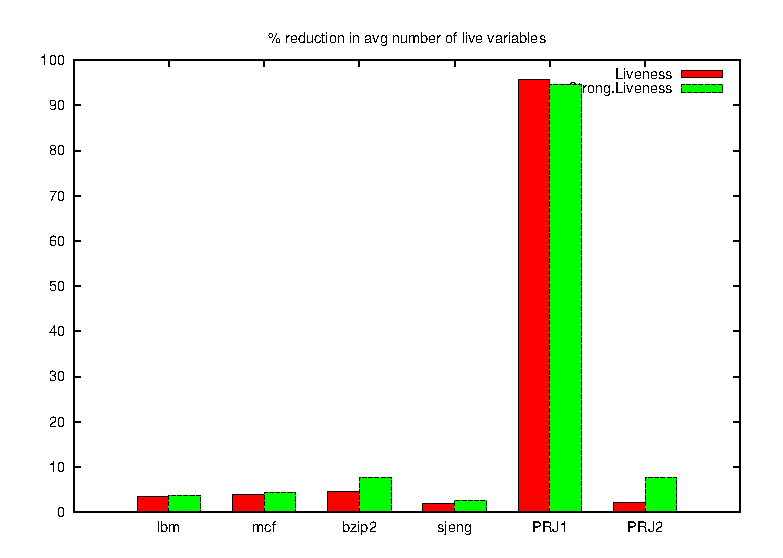
\includegraphics[width=0.8\textwidth]{liveness.eps}
\caption{Percentage reduction in size of live set for context sensitive liveness and strong liveness without aliasing}
\label{fig:liveness}
\end{figure}

\begin{figure}[p]
\centering
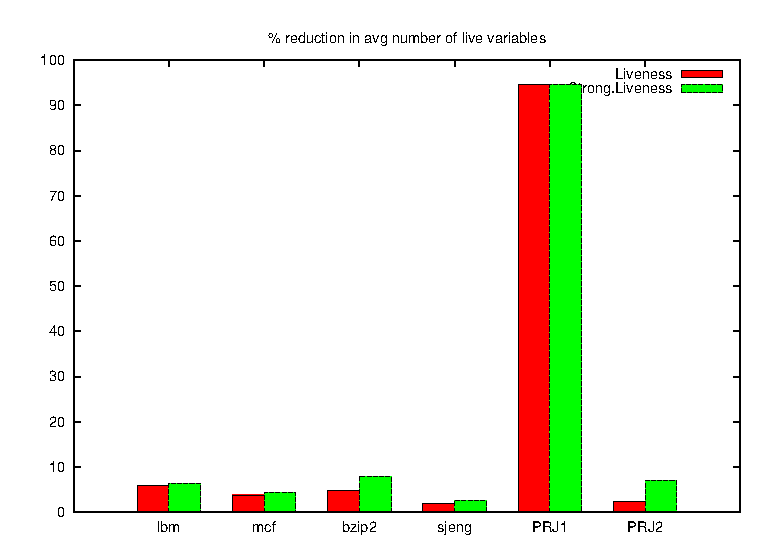
\includegraphics[width=0.8\textwidth]{aliasliveness.eps}
\caption{Percentage reduction in size of live set for context sensitive liveness and strong liveness with aliasing}
\label{fig:livenessalias}
\end{figure}

\begin{figure}[p]
\centering
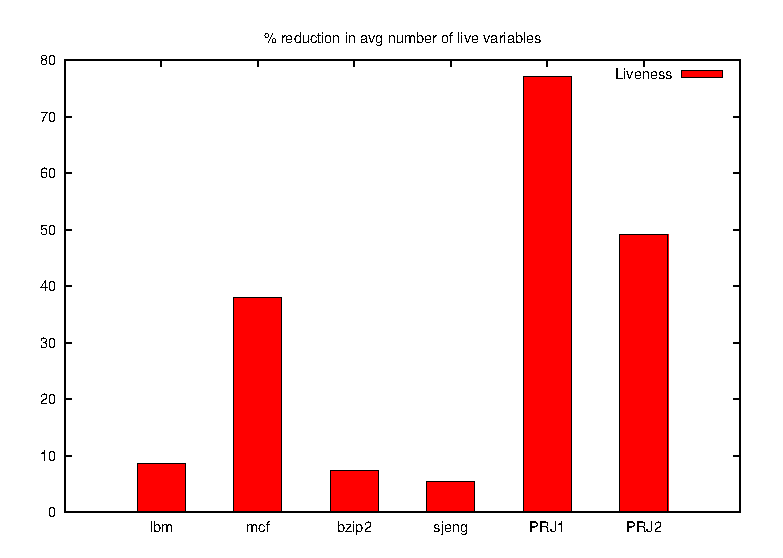
\includegraphics[width=0.8\textwidth]{clive.eps}
\caption{Percentage reduction in size of live set for Context sensitive CLive}
\label{fig:clivelive}
\end{figure}


\section{Measurement of scalability and identifying bottlenecks}

A split up time of various components of the solver was measured to identify bottlenecks. A bottleneck observed var context transition diagram edge retrieval operation. For \emph{bzip2}, it takes 5\% of total solver time. For \emph{PRJ1}, it took 10 \% of total solver time whereas for \emph{PRJ2}, it took 50\% of the total solver time. Thus for more intensive applications, it becomes a dominating factor in deciding the running time. Current implementation of context transition diagram is done using hash maps. A more efficient implementation by using bitmaps can help to remove the bottleneck.
\newpage
\chapter{Future work}

The current solver implemented handles only unidirectional analysis. Moreover it is not fully integrated in PRISM because of which, it does not provide an API access to its results. To fully integrate context sensitive analysis in PRISM we propose the following changes.

\begin{enumerate}
\item The current data structure used for holding results can be viewed as a mapping between program point and data flow value. With contexts sensitive analysis, it needs to be changed to mapping between (program point,calling context) and data flow value.
\item An API needs to be designed for accessing the data flow information for a given context.
\item The kulang specifications need to be changed so that it should include support for specifying Lattice of a data flow problem
\item Based on the lattice, the kulang compiler should generate appropriate flow functions which pass data flow information from one scope to another which can be called by the solver.
\end{enumerate}


We plan to investigate the results obtained on PRJ1 by inspecting the source code of the application.

Once the above specified changes are made, a bidirectional solver can be implemented and context sensitive analysis of bidirectional analyses such as Liveness based Pointer analysis can be implemented in PRISM. A goal of this project is to implement a scalable context sensitive bidirectional framework to solve data flow problems.


\newpage
\appendix
\chapter{User manual of PRISM}
In this section, we present a manual for setting up PRISM on ubuntu system. The first section describes setting up PRISM in eclipse and how to generate an analyzer second section describes how to analyze a program using generated analyzer. An assumption is made that specifications of an analysis are availiable.

\section{Setting up PRISM on Ubuntu and generating the analyzer}
For setting up PRISM involves the following steps

\begin{enumerate}
\item All the locations of all jar files to classpath. It can be done by setting the environment variable CLASSPATH.
\item Create an environment variable PRISMROOT and store in it the url of PRISM root directory.
\item Create a new directory inside \$PRISMROOT/darpan. The name of the directory should be same as name of package as defined in the analysis kulang files. Copy all the analysis specification files to that directory.
\item Run the script populatemodel.sh. This script will create a signature of the analysis.
\item Compile all the kulang files (.klg) with the syntax runKulangC 'filename' . You may have to give execute permissions to the executable runKulangC. It is present in the directory \$PRISMROOT/prism/bin. Upon successful compilation, the generated analyzer would be created and compiled in the same directory.
\item Update the .ini file and all the requires urls. \$PRISMROOT is url of prism root directory. \$PRISMMODEL is the url of signature file Lpum.cdf . The default location of the file is \$PRISMROOT/prism/Models/UserModel/Lpum.cdf. \$REPOSDIR is a location where test results should be dumped. \$IRREPOSDIR is the location from where IR is read.
\item Update the .prj file and set the path of program to be analyzed.
\item Open eclipse, create a new project and import the Driver and Client files of the analysis in the project.
\item Go to project properties--build path--add external jar. Add all the jar files present in \$PRISMROOT/lib.
\item Go to run configurations and create a new run configuration. In the VM arguments section, create an argument -DENVFILE='path of .ini file' In the program arguments give first argument the path of .prj file and second argument the location where test results are to be dumped.
\end{enumerate}

\section{Running an analysis in PRISM using generated analyzer}

This section will describe how an anaysis can be executed in PRISM using generated analyzer.

\begin{enumerate}
\item Write a c program to be analyzer. The name of the front end compiler to be used is cppfe. Compile the file using the command cppfe 'filename' Also give the argument --edg--gcc and -O followed by location where IR should be generated. It should be the same as location of \$IRREPOSDIR given in previous section.
\item For more options of cppfe, use the argument --help to view list of options
\item Go to eclipse and run the Driver file using the run configuration created in the previous section.
\item The results of analysis are by default dumped into .dfi files. These files are created in the location of \$REPOSDIR as specified in the .ini file.
\end{enumerate}


\newpage
\chapter{Kulang queries developed}
The flow functions specified in the kulang specifications of the queries developed are specified in the subsequent sections. The flow function for call statement given in the kulang specification is not executed by context sensitive solver. The context sensitive solver user another flow function which maps variables from caller to calee scope. This flow function is not specified in kulang files. 

\section{Liveness analysis}

Following are the flow functions for liveness anaysis:

\begin{verbatim}
BackwardNodeflow( n: Binary, S: L ) 
let
   rt_expr = rhs( n );
   lt_expr = lhs( n );
   rone = getNEs(rt_expr);
   lone = getNEs(lt_expr);
in
   if (operator (n) == '=')
   then
      (S - lone ) + rone
   else
      (S + lone ) + rone
   endif;

BackwardNodeflow( n: Unary, S: L ) 
let 
   operands_ne = getNEs( n );
in
   S + operands_ne;


BackwardNodeflow( n: Call, S: L ) 
let
   useincall = getNEsFromCall( n );
in
   S + useincall;

BackwardNodeflow( n: Returnstmt, S: L ) 
let
   useinreturn = getNEsFromReturn( n );

in
   S + useinreturn;

\end{verbatim}

\section{Strong Liveness analysis}

For strong liveness analysis, the flow function for assignment statement is different as compared to liveness analysis. Rest of the flow functions are the same. The flow function for assignment statement is given below :

\begin{verbatim}

BackwardNodeflow( n: Binary, S: L ) 
let
   rt_expr = rhs( n );
   lt_expr = lhs( n );
   rone = getNEs(rt_expr);
   lone = getNEs(lt_expr);
   x=	if (operator (n) == '=')
        then
            if(isLive(lt_expr,S)==true)
            then
                 (S - lone ) + rone
            else
                 S
            endif
        else
            (S + lone ) + rone
        endif;
in
   x;

\end{verbatim}

\section{Liveness analysis with aliasing}
The alias closure function used invokes CAlias query and gets alias information from the results of CAlias. The flow functions are given below:

\begin{verbatim}
BackwardNodeflow( n: Binary, S: L ) 
let
   rt_expr = rhs( n );
   lt_expr = lhs( n );
   rone = getNEs(rt_expr);
   lone = getNEs(lt_expr);
   pts = aliasClosure(lt_expr, currentfunction);
   rpts = aliasClosure(rt_expr, currentfunction);
   r = printSet(pts);
   x=  if (operator (n) == '=')
       then
			
          if(isDref(lt_expr) == true)
          then
               if(isMust(pts) == true)
               then				
                   (S - pts) + rone + rpts
               else
                   S + rone + rpts 	
               endif		
          else
               (S - lone) + rone + rpts
          endif 
       else
          (S + lone + rpts + pts) + rone
       endif;
in
    x;

BackwardNodeflow( n: Unary, S: L ) 
let 
   operands_ne = getNEs( n );
   expr_alias = aliasClosure(n, currentfunction);	
in
   S + operands_ne + aliasClosure;


BackwardNodeflow( n: Call, S: L ) 
let
   useincall = getNEsFromCall( n );		
in
   S + useincall;

BackwardNodeflow( n: Returnstmt, S: L ) 
let
   useinreturn = getNEsFromReturn( n );
   expr_alias = aliasClosure(n, currentfunction);

in
   S + useinreturn + expr_alias;

\end{verbatim}

\section{Strong liveness analysis with aliasing}
This is similar to liveness with a difference in flow function for assignment statement. The flow function for assignment statement is given below:

\begin{verbatim}
BackwardNodeflow( n: Binary, S: L ) 
let
   rt_expr = rhs( n );
   lt_expr = lhs( n );
   rone = getNEs(rt_expr);
   lone = getNEs(lt_expr);
   pts = aliasClosure(lt_expr, currentfunction);
   rpts = aliasClosure(rt_expr, currentfunction);
   r = printSet(pts);
   x=   if (operator (n) == '=')
        then
			
            if(isLive(lt_expr,S)== true)
            then
                 if(isDref(lt_expr) == true)
                 then
                      if(isMust(pts) == true)
                      then				
                          (S - pts) + rone + rpts
                      else
                          S + rone + rpts 	
                      endif		
                 else
                      (S - lone) + rone + rpts
                 endif
            else
                 S
            endif
        else
            (S + lone + rpts + pts) + rone
        endif;
in
	x;
\end{verbatim}

\newpage
\bibliographystyle{plain}
\bibliography{Report}
\end{document}


